\documentclass{article}
\usepackage{ctex}
\usepackage[a4paper,left=10mm,right=10mm,top=15mm,bottom=15mm]{geometry}
\usepackage{graphicx}
\usepackage{amsfonts,amssymb}
\usepackage{amsmath}
\usepackage{biblatex}
\usepackage{hyperref}
\usepackage{color}
\usepackage{titlesec}
\usepackage{titletoc}

\title{代码大全笔记}
\author{张谦}
\date{\today}
\begin{document}
\maketitle
\tableofcontents
\newpage

\section{欢迎进入软件构件的世界}
\subsection{什么是软件构建}
如下图所示,构建活动主要是编码与调试,但也涉及详细设计、规划构建、单元测试、集成、集成测试
等其他活动。
\begin{figure}[ht]
    \centering
    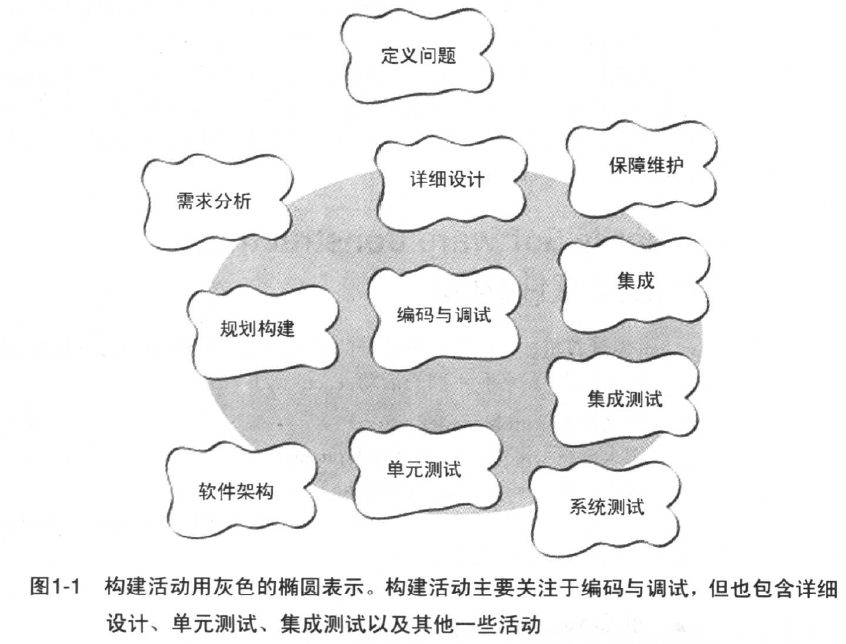
\includegraphics[width=10cm]{figure1.png}
\end{figure}

\par
构建活动包含如下具体任务:
\begin{itemize}
    \item 验证有关的基础工作已经完成,保证构建活动可以顺利进行;
    \item 确定如何测试所写的代码;
    \item 设计并编写类和子程序;
    \item 创建并命名变量和具名常量;
    \item 选择控制结构,组织语句块;
    \item 对代码进行单元测试和集成测试,并排除其中的错误;
    \item 评审开发团队其他成员的底层设计和代码,并让他们评审你的工作;
    \item 优化代码,仔细进行代码的格式化和注释;
    \item 将单独开发的多个组件集成为一体;
    \item 调整代码,让它更快、更省资源。
\end{itemize}

\subsection{构建为什么重要}
\begin{itemize}
    \item 构建活动是软件开发的主要组成部分;
    \item 构建活动是软件开发中的核心活动;
    \item 将主要精力集中于构建活动,可以大大提高程序员生产率;
    \item 构建活动的产物,源代码,往往是对软件的唯一精确描述;
    \item 构建活动是唯一一项确保完成的工作。
\end{itemize}

\section{用隐喻理解软件开发}
隐喻是启示而不是算法,可以将软件开发过程与其他熟悉的活动联系在一起,帮助更好地理解开发过程。
相比其他隐喻,例如写作、种植和养殖等,通过将软件的构建过程,比作房屋的建设过程,能够更好地
理解软件构建的各个阶段。
\subsection{建造隐喻}
\par
(1)问题定义(problem definition):决定准备建一个什么类型的房子;
\par
(2)架构设计(architectural design):和某个建筑师探讨总体设计,并得到批准;
\par
(3)详细设计:画出详细的蓝图,雇一个承包人;
\par
(4)软件构建(construction):准备好建造地点,打好地基,搭建房屋框架,砌好边墙,盖好房顶,
通好水、电、煤气等;
\par
(5)软件优化:在房子大部分完成后,庭院设计师、油漆匠和装修工还要把新盖的房子以及里面的家什
美化一番;
\par
(6)评审和审查(reviews,inspections):在整个过程中,还会有各种监察人员来检查工地、地基、
框架、布线以及其他需要检查的地方。

\subsection{已有组件}
当开发软件时,会大量使用高级语言所提供的功能,而不会自己去编写操作系统层次的代码;
自己编写那些能买得到的现成程序库是没有意义的,例如一些容器类、科学计算函数、用户界面组件、
数据库访问组件等。在建造房子的时候,你也不会去试着建造那些能买得到的东西,例如洗衣机、
冰箱、餐桌等。

\subsection{定制组件}
如果想建造一间拥有一流家具的高档住宅,可能就需要定制的橱柜,以及和橱柜搭配的洗碗机和冰箱等。
在软件开发中也有这种订制的情况,例如想要开发一款一流的软件产品,可能会自己编写科学计算函数,
以便获得更快的速度和更高的精度。

\subsection{防止过度计划}
适当的多层次规划对于建造房屋和构建软件都是有好处的,如果按错误的顺序构建软件,那么编码、测试和
调试都会很难。精心计划,并不是事无巨细的计划或过度计划,例如你可以把房屋的结构性支撑规划清楚,
在日后再决定是用木地板还是瓷砖地板,墙面漆成什么颜色等。

\subsection{不同软件项目}
建筑业中,盖一间仓库或工具房,或是一座医院或核反应站,在规划、设计和质量保证方面所需达到的程度
是不一样的,所用的方法也不相同。同理,在软件开发中,通常只需要用灵活的、轻量级的方法,但有时
你就必须用严格的、重量级的开发方法,以达到所需的安全性目标或其他目标。
另外,还需要特别关注工作时间,在建造帝国大厦时,每辆运料车运输时都留有15分钟的余地,如果
某辆车没能在指定的时间到位,则整个工期就会延误。对于超大型的软件项目,就需要比一般规模的项目
有更高级的规划设计,如果需要创造在经济规模上可以匹敌帝国大厦的庞大软件项目,那么与之相当
水准的技术与管理控制也是必需的。

\section{构建前期准备}
\subsection{前期准备的重要性}
准备工作的中心目标就是降低风险,软件开发中最常见的项目风险是糟糕的需求分析和糟糕的项目计划,
因此准备工作就倾向于集中改进需求分析和项目规划。
高质量的实践方法在项目的初期、中期和末期都强调质量:
\par
(1)如果在项目末期强调质量,那么你会强调系统测试;但是测试只是完整的质量保证策略的一部分,
而且不是最有影响的部分;
\par
(2)如果在项目中期强调质量,那么你会强调构建实践;
\par
(3)如果在项目开始阶段强调质量,那么你就会计划、要求并设计一个高质量的产品;例如你用为吉利车
做的设计来开始整个生产过程,尽管你可以想尽办法来测试,它也绝对不会变成奔驰;也许你能造出最好
的吉利车,但是如果你想要的是奔驰,那么你就得从头开始做设计。

\subsection{序列式开发和迭代式开发选择}
绝大多数的项目都不会完全使用序列式开发法或完全使用迭代式开发法。预先详细说明100\%的需求
和设计是不切实际的,不过对绝大多数项目来说,尽早把那些最关键的需求要素和架构要素确定下来,
时很有价值。
\par
可能因为下列原因选择一个更加迭代的方法:
\begin{itemize}
    \item 需求并没有被理解透彻,或者出于其他理由你认为它是不稳定的;
    \item 设计很复杂,或者有挑战性,或者两者兼具;
    \item 开发团队对于这一应用领域不熟悉;
    \item 项目包含许多风险;
    \item “长期可预测性”不重要;
    \item 后期改变需求、设计和编码的代价很可能比较低。
\end{itemize}
相反的,你可能需要选择一个更加序列的方法。

\subsection{问题定义的先决条件}
在开始构建之前,首先要满足的一项先决条件是,对这个系统要解决的问题做出清楚的陈述。
问题定义只定义了问题是什么,而不涉及任何可能的解决方案。它是一个很简单的陈述,并且听起来
应该像个问题。例如“我们跟不上客户的订单了”听起来就像个问题,而且确实是一个很好的问题
定义;而“我们需要优化数据自动采集系统,使之跟上客户的订单”,这种就是糟糕的问题定义,
它听起来不像问题,而像解决方案。另外,问题定义应该用客户的语言来书写,而且应该从客户的
角度来描述问题。

\subsection{需求的先决条件}
“需求”详细描述软件系统应该做什么,这是达成解决方案的第一步。需求明确有如下好处:
\begin{itemize}
    \item 用户可以自行评审,并进行核准;否则程序员就常常会在编程期间自行决定需求;
    \item 有助于避免争论,如果你和另外一个程序员有分歧,可以查看书面的需求,已解决分歧;
    \item 有助于减少开始编程开发之后的系统变更的情况;
    \item 充分详尽地描述需求,是项目成功的关键,它甚至很可能比有效的构建技术更重要。
\end{itemize}

\par
在构建期间处理需求变更,有以下一些可以采用的方式:
\begin{itemize}
    \item 评估需求质量,如果需求不够好,则停止工作,退回去,先做好后再继续前进;
    \item 确保每一个人都知道需求变更的代价;
    \item 建立一套变更控制程序;
    \item 使用能适应变更的开发方法;
    \item 放弃这个项目;
    \item 注意项目的商业案例,注重商业价值。
\end{itemize}

\subsection{架构的先决条件}
软件架构是软件设计的高层部分,是用于支持更细节设计的框架。架构的质量决定了系统的“概念完整性”,
继而决定了系统的最终质量。一个经过慎重考虑的架构,为“从顶层到底层维护系统的概念完整性”,提供
了必备的结构和体系,它为程序员提供了指引,其细节程度与程序员的技能和手边的工作相配;它将
工作分为几个部分,使多个开发者或多个开发团队可以独立工作。
\par
架构的典型组成部分:
\par
(1)程序组织:
\begin{itemize}
    \item 系统架构首先要以概括的形式对有关系统做一个综述;
    \item 在架构中,应该能发现对那些曾经考虑过的,最终组织结构的,替代方案的记叙;
    找到之所以选用最终的组织结构,而不是其他替代方案的理由;
    \item 架构应该定义程序的主要构造块,根据程序规模的不同,各个构造块可能是单个类,也可能是由
    许多类组成的一个子系统;
    \item 应该明确定义各个构造块的责任,每个构造块应该负责某一个区域的事情,并且对其他构造块负责的
区域知道得越少越好,将设计的信息局限在各个构造块之内;
    \item 应该明确定义每个构造块的通信规则,对于每个构造块,架构应该描述它能直接使用那些构造块,能
间接使用哪些构造块,不能使用哪些构造块。
\end{itemize}

\par
(2)主要的类:
\begin{itemize}
    \item 架构应该详细定义所用的主要的类,应该指出每个主要的类的责任,以及该类如何与其他类交互;
    它应该包含对类的继承体系、状态转换、对象持久化等的描述;如果系统足够大,它应该描述如何将
    这类组织成一个个子系统;
    \item 架构应该记述曾经考虑过的其他类设计方案,并给出选用当前方案的理由;架构无需详细说明
    系统中的每一个类,利用80/20法则:对那些构成系统80\%的行为的20\%的类进行详细说明。
\end{itemize}

\par
(3)数据设计:
\begin{itemize}
    \item 架构应该描述所用到的主要文件和数据表的设计。它应该描述曾经考虑过的其他方案,并说明
    选择当前方案的原因。如果应用程序要维护一个客户ID的列表,而架构师决定使用顺序访问的列表来
    表示该ID的列表,那么文档就应该解释为什么顺序访问的列表比随机访问的列表、堆栈、散列表要好。
    在构建期间,这些信息让你能洞察架构师的思想;在维护阶段,这种洞察力是无价之宝。离开它,你就像
    看一部没有字幕的外语片;
    \item 数据通常只应该由一个子系统或一个类直接访问;例外的情况就是通过访问器类或访问器子程序,
    以受控且抽象的方式来访问数据;
    \item 架构应该详细定义所用数据库的高层组织结构和内容;架构应该解释为什么单个数据库比多个数据库
    要好,反之亦然。需要解释为什么不用平坦的文件,而要用数据库,指出与其他访问同一数据的程序的
    可能交互方式,说明创建哪些数据视图等等。
\end{itemize}

\par
(4)业务规则:
\par
如果架构依赖于特定的业务规则,那么它就应该详细描述这些规则,并描述这些规则对系统设计的影响。例如,
假定要求系统遵循这样一条业务规则:客户信息过时的时间不能超过30秒。在此种情况下,架构就应该描述
这条规则对架构采用的“保持客户信息及时更新且同步”的方法的影响。

\par
(5)用户界面设计:
\par
\begin{itemize}
    \item 用户界面常常在需求阶段进行详细说明,如果没有,就应该在软件架构中进行详细说明。架构
    应该详细定义Web页面格式、GUI、命令行接口等主要元素;
    \item 架构应该模块化,以便在替换为新用户界面时,不影响业务规则和程序的输出部分。例如,架构应该
    使我们很容易做到:砍掉交互式界面的类,插入一组命令行的类。这种替换能力常常很有用,由其
    因为命令行界面便于单元级别和子系统级别的软件测试。1
\end{itemize}

(6)资源管理:
\par
架构应该描述一份管理稀缺资源的计划。稀缺资源包括数据连接、线程、句柄等。在内存受限的应用领域,如
驱动程序开发和嵌入式系统中,内存管理是架构应该认真对待的另一个重要领域。架构应该应该估算在正常情况和
极端情况下的资源使用量。在简单的情况下,估算数据应该说明:预期的运行环境有能力提供所需的资源,
在更复杂的情况下,也许会要求应用程序更主动地管理其拥有的资源。如果是这样,那么资源管理器应该和
系统的其他部分一样,进行认真的架构设计。

\par
(7)安全性:
\par
架构应该描述实现设计层面和代码层面的安全性的方法。如果先前尚未建立威胁模型,那么就应该在架构阶段
建立威胁模型。在制定编码规范的时候,应该把安全性牢记在心,包括处理缓冲区的方法、处理非受信数据
(用户输入数据、cookies、配置数据和其他外部接口输入的数据)的规则、加密、错误信息的细致程度、
保护内存中的秘密数据,以及其他事项。

\par
(8)性能:
\par
如果需要关注性能,就应该在需求中详细定义性能目标。性能目标可以包括资源的使用,这时,性能目标也应该
详细定义资源(速度、内存、成本)之间的优先顺序。架构应该提供估计的数据,并解释为什么架构师相信能
达到性能目标。如果某些部分存在达不到性能目标的风险,那么架构也应该指出来。如果为了满足性能目标,
需要在某些部分使用特定的算法或数据类型,架构应该说清楚。架构中也可以包括各个类或各个对象的
空间和时间预算。

\par
(9)可伸缩性:
\par
可伸缩性是指系统增长以满足未来需求的能力。架构应该描述系统如何应对用户数量、服务器数量、网络节点数量、
数据库记录数、数据库记录的长度、交易量等的增长。如果预计系统不会增长,而且可伸缩性不是问题,
那么架构应该明确地列出这一假设。

\par
(10)互用性:
\par
如果预计这个系统会与其他软件或硬件共享数据或资源,架构应该描述如何完成这一任务。

\par
(11)国际化和本地化:
\par
国际化是一项准备让程序支持多个地域的技术活动。国际化常常称为“I18n",因为国际化的英文单词
“Internationalization”首尾两个字符之间有18个字母。本地化活动是翻译一个程序,以支持当地特定的
语言工作。

\par
(12)输入输出:
\par
输入输出(I/O)是架构中值得注意的另一个领域。架构应该详细定义读取策略是先做、后做还是即时做。
而且应该描述在哪一层检测I/O错误:在字段、记录、流,或者文件的层次。

\par
(13)错误处理:
\par
错误处理已被证实为现代计算机科学中最棘手的问题之一,不能武断地处理它。因为错误处理牵连到整个系统,
因此最好在架构层次上对待它:
\begin{itemize}
    \item 错误处理是进行纠正还是仅仅进行检测?如果是纠正,程序可以尝试从错误中恢复过来。如果
    仅仅是检测,那么程序可以像没发生任何事一样继续运行,也wiagua可以退出。无论哪种情况,都应该通知
    用户说检测到一个错误;
    \item 错误检测时主动的还是被动的?系统可以主动地预测错误,例如,通过检查用户输入的有效性,也
    可以在不能避免错误的时候,被动地响应错误,例如,当用户输入的组合产生了一个数值溢出错误时。
    前者可以扫清障碍,后者可以清除混乱。同样,无论采用哪种方案,都与用户界面有影响;
    \item 程序如何传播错误?程序一旦检测到错误,它可以立刻丢弃引发错误的数据;也可以把这个错误当成
    一个错误,并进入错误处理状态;或者可以等到所有处理完成,再通知用户说在某个地方发现了错误;
    \item 错误消息的处理有什么约定?如果架构没有详细定义一个一致的处理策略,那么用户界面看起来
    就像“令人困惑的乱七八糟的抽象拼贴画”,由程序的不同部分的各种界面拼接而成。要避免这种外观体验,
    架构应该建立一套有关错误消息的约定;
    \item 如何处理异常?架构应该规定代码何时能够抛出异常,在什么地方捕获异常,如何记录这些异常,以及
    如何在文档中描述异常等等;
    \item 在程序中,在什么层次上处理错误?你可以在发现错误的地方处理,可以将错误传递到专门处理
    错误的类进行处理,或者沿着函数调用链往上传递错误;
    \item 每个类在验证其输入数据的有效性方面需要负何种责任?是每个类负责验证自己的数据有效性,
    还是有一组类负责验证整个系统的数据的有效性?某个层次上的类是否能假设它接收的数据是干净的?
    \item 你是希望用运行环境中内建的错误处理机制,还是想建立自己的一套机制?事实上,运行环境
    所拥有的某种特定的错误处理方法,并不是符合你需求的最佳方法。
\end{itemize}

\par
(14)容错性:
\par
架构还应该详细定义所期望的容错种类。容错是增强系统可靠性的一组技术,包括检测错误:如果可能的话,
从错误中回复;如果不能从错误中回复,则包容其不利影响。例如,为了计算某数的平方根,系统的容错
策略有以下几种:
\begin{itemize}
    \item 系统在检测到错误的时候退回去,再试一次。如果第一次的结果是错误的,那么系统可以退回
    到之前一切正常的时刻,然后从该点继续运行;
    \item 系统拥有一套辅助代码,以备在主代码出错时使用。在本例中,如果发现第一次的答案似乎错误,
    系统就切换到另一个计算平方根的子程序,以取而代之;
    \item 系统使用一种表决算法。它可以有三个计算平方根的类,每一个都使用不同的计算方法;
    每个类分别计算平方根,然后系统对结果进行比较;根据系统内建的容错机制的种类,系统可以以
    三个结果的均值、中值或众数作为最终结果;
    \item 系统使用某个不会对系统其余部分产生危害的虚假值代替这个错误的值;
    \item 其他容错方法包括,在遇到错误时,让系统转入某种部分运转状态,或者转入某种功能退化状态;
    系统可以自动关闭或重启。
\end{itemize}

\par
(15)架构的可行性:
\par
设计师关注系统的各种能力,例如是否能达到性能目标,能够在有限的资源下运转,运行环境是否有足够的
支持。架构应该论证系统的技术可行性。如果在任何一个方面不可行,都会导致项目无法实施;那么架构
应该说明“这些问题是如何经过研究的”,通过验证概念的原型、研究或其他手段,必须在全面开展构建之前
解决掉这些风险。

\par
(16)过度工程:
\par
健壮性(robustness)是指系统在检测到错误后,继续运行的能力。通常架构详细描述的系统,会比需求详细
描述的系统更健壮。理由之一为,如果组成系统的各个部分都只能在最低限度上,满足健壮性要求,那么
系统整体上是达不到所有要求的健壮程度的。在软件中,链条的强度不是取决于最薄弱的一环,而是等于所有
薄弱环节的乘积。架构应该清楚地指出程序员应该“为了谨慎起见,宁可进行过度工程(overengineering)”,
还是应该做出最简单的能工作的东西。
\par
详细定义一种过度工程的方法尤其重要,因为许多程序员会出于专业自豪感,对自己编写的类做过度工程。通过
在架构中明确地设立期望目标,就能避免出现“某些类异常健壮,而其他类勉强够健壮”的现象。

\par
(17)关于“买”还是“造”的决策:
\par
如果架构不采用现货供应的组件,那么就应该说明“自己定制的组件,应该在哪些方面胜过现成的程序库和组件”。

\par
(18)关于复用的决策:
\par
如果开发计划提倡使用业已存在的软件、测试用例、数据格式或其他原料,架构应该说明:如何对复用的软件
进行加工,使之符合其他架构目标(如果需要使之符合的话)。

\par
(19)变更策略:
\par
面对变更,软件架构师面临的一个主要挑战,是让架构足够灵活,能够适应可能出现的变化。
\begin{itemize}
    \item 架构应当清楚地描述处理变更的策略。架构应该列出已经考虑过的可能会有所增强的功能,并说明
    “最有可能增强的功能,同样也是最容易实现的”。如果变更很可能出现在输入输出格式、用户交互的风格、
    需求的处理等方面,那么架构就应该说明:这些变更已经被预料到了,并且任何单一的变更都只会影响
    少数几个类。架构应该对变更的计划可以很简单,比如在数据文件中放入版本号、保留一些供将来使用的
    字段、或者将文件设计成能够添加新的表格。如果使用了代码生成器,那么架构应该说明,可预见的变更
    都不会超出该代码生成器的能力范围;
    \item 架构应该指出“延迟提交”所用的策略。比如说,架构也许规定使用表驱动技术。它也许还规定
    “表”中的数据是保存在外部文件中,而非直接写在代码中,这样就能做到在不重新编译的情况下修改程序。
\end{itemize}

\par
(20)架构的总体质量:
\par
优秀的架构规格书的特点在于,讨论了系统中的类、讨论了每个类背后的隐藏信息、讨论了“采纳或排斥
所有可能的设计替代方案”的根本理由。
\begin{itemize}
    \item 架构应该是带有少许特别附加物的,精炼且完整的概念体系。好的架构设计,应该与待解决的
    问题和谐一致;
    \item 在架构开发过程中的多种变更方式,每一项变更,都应该干净地融入整体概念;
    \item 架构的目标应该清楚地表述;
    \item 架构应该描述所有主要决策的动机;
    \item 优秀的软件架构,很大程度上是与机器和编程语言无关的;要尽可能地独立于环境;如果程序
    的用途就是去试验某种特定的机器或语言,那么这条指导原则就不适用了;
    \item 架构应该处于对系统,“欠描述”和“过度描述”之间的那条分界线上;设计者不应该将注意力放在
    某个部件上,而损害其他部件;
    \item 架构应该明确地指出有风险的区域;它应该解释为什么这些区域是有风险的,并说明已经采取了
    哪些步骤以使风险最小化;
    \item 架构应该包含多个视角,包括暴露隐藏的错误和不一致的情况,以及帮助程序员完整地理解系统的设计;
    \item 最后,架构不应该包含任何对你而言,很难理解的东西。
\end{itemize}

\subsection{花费在前期准备上的时间}
花费在问题定义、需求分析、软件架构上的时间,依据项目的需要而变化。一般说来,一个运作良好的项目,
会在需求、架构以及其他前期计划方面,投入$10\%-20\%$的工作量,和$20\%-30\%$的时间。这些时间
不包括详细设计的时间,因为详细设计是构建活动的一部分。


\section{关键的构建决策}
\subsection{选择编程语言}
研究表明,编程语言的选择从多个方面,影响生产率和代码质量。程序员使用熟悉的语言时,生产率比使用
不熟悉的语言时要高。使用高级语言的程序员,能比使用较低级语言的程序员,达到更好的生产率和质量。
每种编程语言都有其优点和弱点,要知道你使用的语言的明确优点和弱点。

\subsection{编程约定}
在高质量的软件中,可以看到“架构的概念完整性”,与“底层实现”之间的关系。“实现”必须与指导该实现的
“架构”保持一致,并且这种一致性是内在的、固有的。这正是变量名称、类的名称、子程序名称、格式约定、
注释约定等这些针对“构建活动”的指导方针的关键所在。在“构建”开始之前,讲清楚你使用的编程约定,
编码约定的细节,要达到这样的精确度:在编写完软件之后,几乎不可能改变软件所遵循的编码约定。

\subsection{深入一种语言去编程}
需要理解“在一种语言上编程”和“深入一种语言去编程”的区别。大多数重要的编程原则,并不依赖于特定的
语言,而依赖于你使用语言的方式。如果你使用的语言缺乏你希望的构件,或者倾向于出现其他种类的问题,
那就应该试着去弥补它,发明你自己的编码约定、标准、类库以及其他改进措施。

\section{软件构建中的设计}
软件设计是指构思、创造或发明一套方案,把一份计算机软件的规格说明书要求,转变为可实际运行的软件。
设计就是把需求分析和编码调试连接在一起的活动。好的高层设计能提供一个可以稳妥容纳多个较低层次设计
的结构。
\subsection{设计中的挑战}
(1)设计是一个Wicked问题:
\par
Wicked问题是指那种只能通过解决或部分解决才能被明确的问题。你必须首先把这个问题“解决”一遍,
以便能够明确地定义它,然后再次解决该问题,从而形成一个可行的方案。例子,有一座桥,设计时主要
考虑的问题为是否足够结实,以承受设计负荷;没有意识到大风带来的横向谐波,最终导致大桥坍塌。

\par
(2)设计是一个了无章法的过程:
\par
软件设计的成果应该是组织良好、干净利落的,然而形成这个设计的过程,却并非如此清爽。
\begin{itemize}
    \item 在设计过程中你会采取很多错误的步骤,多次误入歧途。事实上,犯错正是设计的关键所在,
    在设计阶段犯错并加以改正,其代价要比在编码后才发现同样的错误,并彻底修改低得多;
    \item 优劣设计之间的差异,往往非常微妙;
    \item 很难判断设计何时算是“足够好”了。
\end{itemize}

\par
(3)设计是确定取舍和调整顺序的过程:
\par
设计的一个关键内容,是去衡量彼此冲突的各项设计特性,例如存储空间、占用的网络带宽、时间成本等。

\par
(4)设计涉及到诸多限制
\par
设计的要点,一部分是在创造可能发生的事情,而另外一部分又是在限制可能发生的事情。如果人们在建造房屋时,
拥有无限的时间、资源和空间,那么你会看到房屋不可思议地随意蔓延,每幢楼都有上百间屋子,一只鞋
就可以占用一间屋子。

\par
(5)设计是不确定的:
\par
如果让三个人去设计一套同样的程序,可能会有三套截然不同的设计。

\par
(6)设计是一个启发式过程:
\par
因为设计充满了不确定性,因此设计也就趋于具有探索性,而不是保证能产生预期结果的课重复过程,
设计过程中总会有试验和犯错误。

\par
(7)设计是自然而然形成的:
\par
设计是在不断地设计评估、非正式讨论、写试验代码以及修改试验代码中演化和完善的。

\subsection{关键的设计概念}


\section{可以工作的类}

\section{高质量的子程序}

\section{防御式编程}

\section{伪代码编程过程}

\section{使用变量的一般事项}

\section{变量名的力量}


\section{基本数据类型}

\section{不常见的数据类型}

\section{组织直线型代码}

\section{条件语句}

\section{控制循环}

\section{不常见的控制结构}

\section{表驱动法}

\section{一般控制问题}

\section{软件质量概述}

\section{协同构建}

\section{开发者测试}

\section{调试}

\section{重构}

\section{代码调整策略}

\section{代码调整技术}

\section{程序规模对构建的影响}

\section{管理构建}

\section{集成}

\section{编程工具}

\section{布局与风格}

\section{自说明代码}

\section{个人性格}

\section{软件工艺}

\section{更多信息}


\begin{thebibliography}{99}  
    \bibitem{Meyer2000}Meyer CD (2000) Matrix Analysis and Applied Linear Algebra. Philadelphia, PA: SIAM.
    \bibitem{consistency} Agostino Martinelli. Closed-form solution of visual-inertial structure from motion. International
    Journal of Computer Vision, Springer Verlag, 2013. ￿hal-00905881
\end{thebibliography}



\end{document}

